\subsection{音声認識システムの流れ}
音声認識の流れを図\ref{fig:flow_sp}に示す。まず、入力された音声データから前処理として雑音区間と無音区間を除去し、発話区間を検出する。次に検出した発話区間の音響的特徴量を抽出し、デコーダへと渡す。デコーダではこの音響的特徴量をもとに、音響モデルと言語モデル、単語辞書を参照しながら単語列の尤度を算出し、最も尤度の高いものを認識結果として出力する。言語モデルと単語辞書については\ref{language_model}節、音響モデルについては\ref{acoustic_model}節で説明する。

\begin{figure}[H]
  \begin{center}
    \includegraphics{../../image/flow_sp.eps}
  \end{center}
  \caption{音声認識の流れ}
  \label{fig:flow_sp}
\end{figure}

\subsection{単語辞書と言語モデル}
\label{language_model}

\noindent{\textbf{\underline{単語辞書}}}\par
単語辞書には、一般的に学習データに出現する単語のなかで出現頻度の高い単語を登録する\cite{sp_recognition_shikano}。言語モデルもその単語辞書に登録された単語を用いて構築する。単語辞書の例を表\ref{table:tango}に示す。単語辞書には表記、発音形、原型、品詞番号、出現表記、音素表記などを登録する。\par

\begin{table}[H]
  \begin{center}
    \caption{単語辞書の例}
    \begin{tabular}{|c||c|c|} \hline
      表記+発音形+原形+品詞番号 & 出力表記 & 音素表記 \\ \hline
      あか+アカ+アカ+14 & あか & a k a \\ \hline
      技術+ギジュツ+ギジュツ+1 & 技術 & g i zh j u ts u \\ \hline
      新聞+シンブン+シンブン+1 & 新聞 & sh i ng b u ng \\ \hline
    \end{tabular}
    \label{table:tango}
  \end{center}
\end{table}

音声認識では、言語モデルは、「表記+発音形+原型+品詞番号」を、音響モデルは「音素表記」の部分を用いて最尤の単語を算出する。辞書に登録している単語が少ない場合、入力された単語が辞書に登録されていないことが多くなり、他の誤った単語を出力し認識率が低下してしまう。一方、辞書に登録している単語が多すぎる場合、認識処理に時間がかかるだけでなく、認識候補が増えるため認識率が低下してしまう。よって適切な単語の登録数を検討する必要がある。\vspace{0.2in}

\noindent{\textbf{\underline{言語モデル}}}\par
音声認識における言語モデルとは、文の品詞や単語と単語の関係性、音素の並びの制約などを定式化したもののことである。言語モデルの主流はサンプルデータから統計的な手法によって確率推定を行なう統計的言語モデルである。その中でも最も広く使われているのが$N$グラムモデルである。\vspace{0.2in}

\noindent{\textbf{\underline{$N$グラムモデル}}}\par
$N$グラムモデルとは、与えられた単語列$\omega_1,\omega_2,\cdots,\omega_n$に対して、その出現確率$p(\omega_1,\omega_2,\cdots,\omega_n)$を推定する場合に、

\begin{equation}
P(\omega_1,\omega_2,\cdots,\omega_n)=\prod_{i=1}^{n}p(\omega_{i}\mid \omega_{i-N+1}\cdots \omega_{i-1})
\end{equation}

のような近似を行なうモデルである。$N$グラムモデルでは、$i$番目の単語$ω_i$の生成確率が、直前の$N-1$単語$ω_{i-N+1}\cdots ω_{i-2}ω_{i-1}$だけに依存すると考える。特に$N = 1$のときユニグラム(unigram)、$N = 2$のときバイグラム(bigram)、$N = 3$のときトライグラム(trigram)という。\par
文や発話中の単語の生成確率は文脈に依存することから、$N$グラムモデルの推定確率は、$N$が大きいほど高くなる。しかし、$N$グラムモデルは語彙の$N$乗のコストがかかることから、$N$を大きくするためには、膨大な量のテキストを用意しなければならない。しかし、自由発話を記述したテキストは極めて少ない。本研究では、$N = 3$のtrigramを用いる。\par



\subsection{音響モデル}
\label{acoustic_model}
音響モデルとは、音声の最小単位である音素または、単語や音節の音響特徴パラメータの時系列をモデル化したものである。この音素の特徴は、発話者や発話内容などによって変化するが、発話者ごと、または発話タスクごとにモデル化することは、膨大なコストがかかり汎用性がないため好ましくない。そのため、音響モデルの構築方法としては、音素ごとに様々な学習音声で学習を繰り返し、最尤の音響モデルを作ることが一般的である。本研究では、隠れマルコフモデル(Hidden Markov Model)を用いて最尤の音響モデルを構築する。\par
以下に音響モデルを構築する際に、必要となる知識について述べる。\vspace{0.2in}

\noindent{\textbf{\underline{MFCC}}}\par
メル周波数ケプストラム係数(Mel - Frequency Cepstrum Coefficient : MFCC)とは、メル周波数という人間の音の高低に対する感覚尺度で音声スペクトルから係数スペクトルを抽出したものである\cite{sp_recognition_shikano}。これは一般的に、音声の特徴を抽出するパラメータとして用いられる。
 MFCCの計算では、スペクトル分析は周波数軸上に$L$個の三角窓を配置し、フィルタバンク分析により行なう。すなわち、窓の幅に対応する周波数帯域の信号のパワーを、単一スペクトルチャネルの振幅スペクトル $|S^\prime (k)|$ の重み付けの和$m(l)$ で求める。

\begin{equation}
m(l)=\sum_{k=lo}^{hi}W(k;l)\mid S^\prime(k)\mid \quad (l=1,\cdots,L)
\end{equation}

\begin{equation}
W(k;l)=\begin{cases}\frac{k-k_{lo}(l)}{k_c(l)-k_{lo}(l)}\quad \{k_{lo}\leq k \leq k_c(l)\} \\\frac{k_hi(l)-k}{k_{hi}(l)-k_{l}(l)}\quad \{k_{c}\leq k \leq k_{hi}(l)\} \end{cases}
\end{equation}

ただし、$W(k;l)$ は重み、$k_{lo}(l)、k_c(l)、k_{hi}(l)$ はそれぞれ$l$番目のフィルタの下限、中心、上限のスペクトルチャネル番号であり、隣り合うフィルタ間で

\begin{equation}
k_c=k_{hi}(l-1)=k_{lo}(l+1)
\end{equation}

なる関係がある。さらに、$k_c(l)$はメル周波数軸上で等間隔に配置される。メル周波数は

\begin{equation}
Mel(f)=2595\log_{10}(1+\frac{f}{700})
\end{equation}

により計算される。ただし、$f$の単位は[Hz]にとる。\par
最終的にフィルタバンク分析により得られた$L$個の帯域におけるパワースペクトルを離散コサイン変換することで、式(\ref{eq:mfcc})のようにMFCCが得られる。

\begin{equation}
\label{eq:mfcc}
c_{mfcc}(i)=\sqrt{\frac{2}{N}}\sum_{i=1}^{L}\log ml \cos \left\{ \left( l-\frac{1}{2}\frac{i\pi}{L} \right)\right\}
\end{equation}

\vspace{0.2in}
\noindent{{\textbf{\underline{隠れマルコフモデル(HMM)}}}\par
HMMは時系列信号の確率モデルであり、複数の定常信号源の間を遷移することで、時系列に適応させ、音響モデルを構築する\cite{sp_recognition_shikano}。図\label{fig:HMM}にHMMの例を示す。a,b,cは状態、矢印は状態遷移を示す。HMMは次の状態への遷移と現在の状態の遷移を行なう。このように現在の状態への遷移があるため、様々な長さの時系列信号に対応できる。

\begin{figure}[H]
  \begin{center}
    \includegraphics{../../image/HMM.eps}
  \end{center}
  \caption{HMMの例}
  \label{fig:HMM}
\end{figure}

\noindent{{\textbf{\underline{調音結合}}}\par
音素の音響的な特徴は、周辺前後の音素の影響を受けて同じ音素でも様々に変化することが知られている\cite{sp_recognition_shikano}。この現象を調音結合という。特に、音素から音素への渡りの部分ではスペクトル特徴が時間とともに連続して大きく変化するため、音声を扱う分野ではこの調音結合への対応が重要である。この調音結合に対する最も直接的な対応策として、前後の音素を考慮した3つ組音素(トライフォン)を認識の処理単位として用いるものがある。\par
MFCCは、フレームと呼ばれる数十ms程度の音声区間を定常とみなした上で得られる静的な特徴量である。しかし調音結合があるため、フレーム分析により得られた静的な特徴に加え、時間とともに変化する動的な特徴を特徴量に加えて音声認識を行なうことで、認識の精度が大きく向上することが知られている。動的な特徴には式\ref{eq:deltac}や式\ref{eq:deltadeltac}で示される一次差分か二次差分を利用することが多い。ここで、$K$は回帰係数を計算する範囲であり、一般的に20$\sim$40msである。

\begin{equation}
\label{eq:deltac}
\Delta c(n;l)=\frac{\Sigma_{K=-K}^{K}k_c(n;l+k)}{\Sigma_{K}^{K=-K}K^2}
\end{equation}

\begin{equation}
\label{eq:deltadeltac}
\Delta\Delta c(n;l)=\frac{\Sigma_{K=-K}^{K}k_c(n;l+k)}{\Sigma_{K}^{K=-K}K^2}
\end{equation}
\subsection{DNNの概要}
本研究ではDNNをベースとした会議音声認識を行なう。DNNとは、多層ニューラルネットワークを使った機械学習のことである。DNNは図\ref{fig:dnn}のように、auto-encoderまたはRestricted Boltzmann Machines (RBM)などを積み重ねた深い構造をもつ。入力に近い層では、単純に特徴抽出しかできないが、それらの重み付け和をとると表現能力が上がり、それをさらに上位の層の入力にしていくことで、モデルの表現力がさらに上がるとされている。\par

\begin{figure}[H]
  \begin{center}
    \includegraphics{../../image/image_dnn.eps}
  \end{center}
  \caption{DNNの構造図}
  \label{fig:dnn}
\end{figure}

音声認識においては、入力層の入力はMFCCなどの音響特徴量となり、出力層はHMMの各状態となる。

\subsection{モデルの構築手順}}}\par
DNNを用いた音響モデルの構築や、この音響モデルを用いた音声認識に必要な学習テキストや言語モデルを作成する為にKaldiツールキット\cite{kaldi}を用いた。このツールキットの大きな流れを図\ref{fig:flow_train_dnn}に示す。まず学習や評価に必要なデータを用意し、言語モデルと単語辞書のWeighted Finite State Transducer (WFST)を作成する。WFSTとは重み付き有限トランスデューサといい、状態遷移機械モデル有限オートマトンの一種である。次に音声データから特徴量を抽出したデータを準備し、このデータと書き起こしを用いてGMM-HMMによる音響モデルのWFSTを作成する。これらのWFSTを、合成等を行ない1つのWFSTとする。このWFSTを用いて音声認識を行ない、学習データのアライメント(フレームごとの音素情報)をとる。このアライメントを用いてDNNを用いた音響モデルの学習(プレトレーニングと微調整)を行ない、最終的な音声認識を行なう。

\begin{figure}[H]
  \begin{center}
    \includegraphics{./figure/flow_train_dnn.eps}
  \end{center}
  \caption{DNNを用いる際の学習の流れ \label{fig:flow_train_dnn}}
\end{figure}


